%
% Transportation Research Board conference paper template
% version 3.1 Lite
%
% When numbered option is activated, lines are numbered.
\documentclass[numbered]{trbunofficial}
\usepackage{graphicx}
%\usepackage{cite}
\usepackage{amsmath,amssymb,amsfonts}
\usepackage{algorithmic}
\usepackage{graphicx}
\usepackage{textcomp}
\usepackage{xcolor}
\usepackage{multirow}
\usepackage{pdflscape}
\usepackage{afterpage}
\def\BibTeX{{\rm B\kern-.05em{\sc i\kern-.025em b}\kern-.08em
    T\kern-.1667em\lower.7ex\hbox{E}\kern-.125emX}}

% \usepackage[colorlinks=true,linkcolor=blue,citecolor=blue]{hyperref}
% For TRB version hide links
\usepackage[hidelinks]{hyperref}

\makeatletter
\renewcommand\@biblabel[1]{#1.}
\makeatother

% Put here what will go to headers as author
\AuthorHeaders{Brown, Garikapati and Hou}
\title{A Machine Learning Decision Support Tool for\ \ \ \ \ \ \ \ \ \ \ \ \ \ \ \ \ \ \ \ \ \ \ \ \ \ \ \ \ \ \ \ \ \  Travel Demand Modeling}

% TODO: add macros for easier formatting of \author.
\author{%
  \textbf{CScott Brown}\\
University of South Alabama\\
Email: gitpushoriginmaster@gmail.com\\
  \hfill\break%
  \textbf{Venu M. Garikapati, Ph.D}\\
National Renewable Energy Laboratory\\
15013 Denver West Parkway, Golden, Colorado 80401\\
Tel: 303-275-4784\\
Email: venu.garikapati@nrel.gov\\
  \hfill\break% this is a way to add line numbering on empty line
  \textbf{Yi Hou}\\
National Renewable Energy Laboratory\\
15013 Denver West Parkway, Golden, Colorado 80401\\
Tel: 303-384-7525\\
Email: yi.hou@nrel.gov \\
}

% If necessary modify the number of words per table or figure default is set to
% 250 words per table and figure
% \WordsPerTable{250}
% \WordsPerFigure{250}

% If words are counted manually, put that number here. This does not include
% figures and tables. This can also be used to avoid problems with texcount
% program i.e. if one does not have it installed.
\TotalWords{6995}

\begin{document}




\maketitle



\section{Abstract}
Utility maximization models are the lifeblood of virtually all travel demand models in practice. 
 Be it the traditional travel demand models or more advanced activity-based models, utility maximization models are used extensively to model and predict myriad travel choices such as location choice, mode choice and route choice. 
 There has recently been increased interest in incorporating machine learning into travel demand models where they can enhance prediction accuracy. 
 Though there have been sporadic efforts at comparing specific utility maximization models to machine learning models, there is a need for a standard comparison tool which can evaluate machine learning models against utility maximization models for a given choice context. 
 Addressing this need, we present a tool for applying an array of models including logit, nested logit, neural network, Naive Bayes and decision tree classifiers. 
 The tool is designed to be easily extensible, accounts for common pitfalls in the application of various models, automatically selects optimum hyperparameters and reports a variety of metrics commonly employed to evaluate model performance. 
 The tool is specifically tailored to aid in deciding the best model for a given choice context and can be used to choose an appropriate model family or to construct a model ensemble. 
 We test our proposed system on household vehicle count and work schedule targets from the 2017 National Household Travel Survey. 
 Results demonstrate that for some variables, logit are not the most effective models, and the proposed system can aid in selecting a better model.

\hfill\break%
\noindent\textit{Keywords}: Utility Maximization, Machine Learning, Decision Support Tool, Travel Demand Modeling
\newpage

\section{Introduction}\label{section:introduction}
Logistic regression has long been the golden standard for classification modeling in transportation problems.
 State-of-the-art transportation simulation software \trbcite{horni2016multi, sheppard2017modeling} in use by departments of transportation around the globe have at their core this tried-and-true family of functions.
 However, as available data grows in size and scope and desired models move from aggregate trip-based to more intricate activity-based designs, models are being required to capture increasingly complex relationships between variables.
 It is not clear if the restrictive assumptions accompanying logistic regression remain valid in this increasingly complex domain.
 
Despite a wealth of work demonstrating situations in which alternative model families can produce superior results, adoption of alternative model families amongst transportation practitioners remains low.
 Partly this is accounted for by the simplicity of interpretation of logit models and the fact that they are so deeply ingrained in the current tools for travel demand modeling.
 Further, most travel demand modeling problems involve a great number of models for a variety of parameters.
 For example, the Comprehensive Econometric Micro-simulator for Daily Activity-travel Patterns (CEMDAP) \trbcite{pinjari2008cemdap} involves at least 57 separate models, 26 of which are logit models, most of the remainder being regression or ordinal probit.
 For any problem, there are a great many possible model families that can be applied, and it is a priori unclear whether investing in the development of more complex models will be valuable for a given set of predictors and targets.
 Finally, applying different families of models can involve a range of necessary preprocessing steps and implementation pitfalls that can make casting a final judgement between one model family or another difficult.

Recently, machine learning (ML) models are being adopted in various domains and have been shown to be more accurate than traditional models at many tasks. 
 ML is a subfield of computer science that enables machines to learn patterns or rules from data without being explicitly programmed. 
 In the transportation field, ML is gaining rapid popularity in driver behavior modeling \trbcite{meng2012classification}, travel time prediction \trbcite{hou2017road}, traffic forecasting \trbcite{ma2015large}, volume estimation \trbcite{hou2018network}, and safety analysis \trbcite{brijs2007bayesian, miranda2007bayesian}. 
 ML techniques often require less stringent assumptions on, for example, variable distributions than traditional statistical modeling methods.
 As a result, ML models are capable of capturing the underlying relationships among different variables in an environment of uncertainty even when they are not easily apparent. 
 Nevertheless, like any other modeling tool, there are some concerns for ML models. 
 Some ML paradigms lack good interpretations of the models and are usually seen as a ``black box'' approach. 
 Also, many ML models demand more computational resources than traditional statistical models.
 
Given existing barriers to replacing logit models with more robust alternatives, we propose a modeling pipeline to apply an array of ML algorithms alongside logit models to provide practitioners with a simple yet effective means of gauging the predictive abilities of utility maximization and ML algorithms for a given modeling context.
 It should be noted that the intent of this research is not to decide or critique which modeling technique is superior, but simply to develop a decision support tool that can bring the best of both utility maximization and ML worlds to benefit the state of practice in travel demand modeling.
 We believe that the ability to choose an appropriate model family for each of the great number of individual problems in travel demand modeling will improve the predictive power of overall models and the resulting simulations.
 Furthermore, in situations where interpretability is not a concern, a set of models can be ensembled to create a model that accounts for the inevitable shortcomings of each family resulting in a single more robust model.

In the proceeding sections, we test the capabilities of the proposed system on two case studies from NHTS 2017.
 The goals of our experiments are the following:
 First, to examine the hypothesis that standard modeling pipelines can be applied to a variety of problems and provide reasonable models to facilitate model family performance comparison.
 Such a pipeline is important, since different model families may be subject to different data preprocessing considerations such as hyperparameter selection, feature selection, class balance and variable scaling.
 Second, to provide a tool, TEAM-TDM (A Tool for Evaluating an Array of ML Travel Demand Models) that automates the entire process, allowing practitioners to effortlessly evaluate a range of model families on a variety of problems and datasets.
 
The remainder of the paper is organized as follows.
Section \ref{section:related_work} reviews research demonstrating the value of various ML algorithms in transportation modeling.
Section \ref{section:methodology} describes the proposed array of models, and lays out the order, means and reasonings behind the experiments performed.
Section \ref{section:results} summarizes the results of our experiments.
Finally, section \ref{section:conclusions} discusses important takeaways, limitations and future work.

\section{Related Work}\label{section:related_work}

In this section we review research evaluating the relative performance of logit regression (MNL) and ML algorithms for classification in transportation problems.
 We attempt to provide diverse and popular exemplars of the subject, covering the most common model families, and especially focusing on works that evaluate multiple models.
 Commonly applied model families (besides logit) include support vector machines (SVM), multi-layer perceptrons (MLP) (a subset of neural networks (NN)), naive bayes (NB), decision trees (DT) and various derivatives such as bagged and boosted varieties, and other model ensembles.
 NN models are the most commonly evaluated model family in the literature, and an entire review \trbcite{karlaftis2011statistical} is dedicated to NNs vs classical statistical models (including MNL) for transportation problems.

Mode choice is by far the most popular target variable for evaluating model families, despite the fact that alternative model families repeatedly demonstrate mediocre gains in performance vs MNL models for this problem.
 Zhang et al \trbcite{zhang2008travel} perform a comparison of SVM, MLP and MNL models for mode choice modeling.
 Notably, they compare against a known and thoroughly vetted MNL model, painstakingly conceived and refined in \trbcite{koppelman2006self} to even include non-linear variable combinations.
 All three models perform comparably, with the SVM model having a slight edge, even without having included the same non-linear variable combinations fed to the MNL model.
 Xie et al \trbcite{xie2003work} compare DT, MLP and MNL models also for mode choice.
 All three modes again perform comparably, with the DT and MLP models performing slightly better.
 The authors point out the interesting observation that an MNL model is actually a special case of MLP, and also point out the problem of class balance in training certain types of classifier in a transportation context.
 Vythoulkas et al \trbcite{vythoulkas2003modeling} also compare MNLs with a NN architecture but go to great lengths to develop a NN architecture that captures various decision structures hypothesized to be analagous to natural human reasoning.
 Even so, the NN and logistic regression models perform comparably.
 Hagenauer et al \trbcite{hagenauer2017comparative} compare a number of model families, including MNL, MLP, DT, several ensemble varieties of DT, NB, and SVM using the Dutch National Travel Survey.
 Interestingly, they observe a performance difference between MNL and other models that is significantly greater than observed in previous studies, with random forests achieving upward of $90\%$ accuracy.
 The reason for this distinction is unclear.
 However, this suggests hope that in some circumstances a comparison tool for an array of models may distinguish situations where alternatives to MNL models shine.

Since MNL is so ingrained in transportation modeling culture, other target variables for evaluating the performance of MNL vs ML methods span the gamut of topics related to transportation.
 Mohammadian and Miller \trbcite{mohammadian2002nested} compare a nested MNL with NNs for modeling vehicle ownership.
 They find that the NN gives a better accuracy for individual predictions but note that there are a variety of metrics by which models might be compared, including aggregate market share and log loss.
 Park et al \trbcite{park2007learning} compare MNL and DT models for route choice modeling.
 The models perform comparably on their dataset, with the DT model notably performing quite well even when utility maximizing (MNL-generated) routes were taken to be ground truth.
 Allahviranloo and Recker \trbcite{allahviranloo2013daily} compare MNL and SVM models for predicting daily activity sequences.
 Although the MNL performs slightly better for predicting the initial activity of the day, the SVM model is significantly better at predicting subsequent activities.
 Clark \trbcite{clark2009determinants} compares NB and DT models for predicting vehicle ownership rates, and provide some discussion comparing their results with those of other studies employing MNL models.
 They also find little difference in the predictive capabilities of ML models and more classical approaches.
 However, they do note that the NB model is particularly good at classifying certain classes, which suggests that an ensemble of models may be viable.

Many other works focus entirely on MNL models solely, or on some other specific model family.
 Despite the large corpus of work applying ML models to transportation problems, the studies are difficult to compare, owing to models having been built on diverse datasets and with different designs concerning model hyperparameters, data preprocessing, etc.
 Furthermore, all of the above studies were conducted with the intention of constructing the best possible model for a given problem, rather than creating a tool that can be applied to a variety of problems.
 Through this research effort, we address these concerns by using TEAM-TDM to compare a wider range of model families than most previous studies, that can be applied with little or no alteration to different datasets to provide maximum consistency between studies.
 We also show that TEAM-TDM can be quickly and easily adapted to new problems, allowing practitioners and researchers to easily and fairly compare the performance of different model families on individual tasks.

\section{Methodology} \label{section:methodology}

In this section we describe the exact set of models and related data processing pipeline comprising our experiments with TEAM-TDM and the reasonings behind individual choices.
 First, we provide a brief overview of the applied models, expected benefits and shortcomings of each, as well as references for a more detailed understanding of the related mathematics.
 Also, we examine the training procedures, data (pre)processing and hyperparameter selection.
 Figure \ref{fig:flowchart} outlines the general structure of the TEAM-TDM pipeline.
 Finally, we outline the experiments that we will perform and the datasets upon which we will apply our models.

\begin{figure}[!ht]
  \centering
  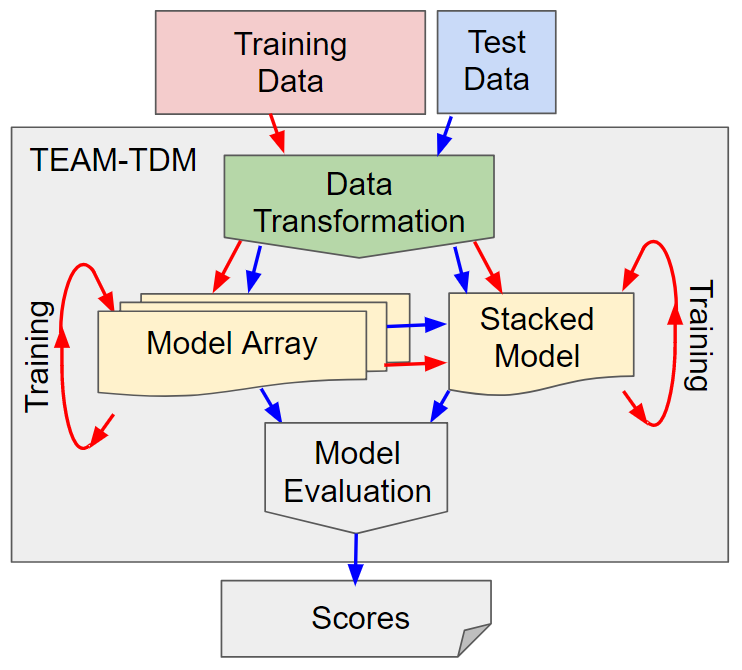
\includegraphics[width=0.6\textwidth]{flowchart}
  \caption{The TEAM-TDM tool.}\label{fig:flowchart}
\end{figure}

\subsection{Models} \label{subsection:models}

The models we evaluate in our expereiments with TEAM-TDM include logit (MNL), random forests (RF), multi-layer perceptrons (MLP) and naive bayes (NB).
 We also include other models when appropriate, such as ordered probit (OP) and nested logit models (NL) to demonstrate the ease with which additional models can be added to TEAM-TDM when desired.

Logit models \trbcite{berkson1944application} are statistical models that are the traditional standard for classification problems, being some of the earliest model families for classification.
 MNL are linear models, in the sense that MNL models can only be $100\%$ effective on data that are perfectly linearly separable.
 Also, MNL models assume that, for multi-class problems, the choice between any pair of alternatives is independent of the distribution of other alternatives.
 This is referred to as the independence of irrelevant alternatives assumption (IIA), and, when problematic, is sometimes addressable by `nesting' logit models \trbcite{mcfadden1978modeling}.
 Despite these restrictive assumptions, MNL models enjoy broad success in a wide range of applications, due to the fact that many datasets satisfy the assumptions at least approximately and because the learned parameters of an MNL model can often be interpreted easily.
 In TEAM-TDM, we include a simple MNL model without regularization.

Decision trees \trbcite{quinlan1986induction} are a popular class of models due to their speed in both training and prediction, ready interpretability and general ease-of-use.
 A DT model performs a classification by recursively choosing a feature and then `deciding' a branch of the tree based on the value of that feature until a prediction can be made on the target variable.
 The training procedure for a DT model family consists of finding a tree so that the series of `decision' branches results in accurate predictions.
 Choosing the optimal decision tree from the set of all possible trees is known to be an NP-complete problem.
 As such, various methods exist for choosing an optimal tree from some subset of all possible trees.
 We employ CART \trbcite{breiman1984classification}, which creates branches based on the criterion of Gini Importance.
 DT models have a number of known issues, including a tendency to overfit without considerable supervision.
 One popular method of dealing with the overfitting issue, known as a random forest (RF) \trbcite{ho1995random}, is to construct an ensemble of weak decision trees each trained on a random subset of the data.
 This trades in speed and interpretability for a more robust classifier.
 In TEAM-TDM, we include an RF classifier where the depth of the individual trees is an optimized hyperparameter.

Multi-layer perceptrons \trbcite{rumelhart1985learning} can be seen as a simple extension of MNL.
 MNL applies a linear transformation to the features from $n$ feature dimensions into $m$ target class dimensions, followed by a softmax ``activation'' function to obtain probability-esque output.
 It is entirely possible to chain these functions to obtain a more complex decision surface.
 Such a chaining process is the basic thought behind MLP models, and can be done to arbitrary depths, and with arbitrary activation functions.
 The benefit of MLPs over MNLs is their ability to model non-linear decision boundaries, at the cost of less interpretability, slower training/prediction speeds, and a danger of overfitting, especially for very deep MLPs.
 In TEAM-TDM, we include an MLP with one hidden layer, rectified linear unit activations and $L_2$ regularized weights, where the number of `hidden' dimensions $h$ is an optimized hyperparameter, always trained for a fixed 1000 epochs.

Naive Bayes is a simple family of models that makes an assumption that the feature values are all independent conditioned on the target value.
 Thus, we can predict the probability of a target class given each feature value independently based on the distribution of the training data.
 For continuous valued features, we make a further assumption that the feature values are Gaussian distributed.
 For discrete valued features, we simply use the empirical distribution.

Ordinal regression problems, which occupy an intermediate ground between classification and regression can be handled in a number of ways.
 One common method is to simply cast the problem as a classification problem.
 Other methods comprise inclusion of latent variables to measure the varying degrees of separation characterized by ordinal problems, or by nesting classifiers in a one vs rest tree to cast the ordinal regression as a series of binary classification problems \trbcite{frank2001simple}.
 Since these types of problems appear frequently in transportation modeling, we provide an option in the Pipeline for including them when appropriate.
 In TEAM-TDM, we include an OP and also an NL where nests are constructed into a tree of binary problems $y = i$ vs $y > i$.

Finally, for reference, we include a stratified dummy classifier which randomly predicts a class according to the empirical distribution of classes in the training data without regard to any features.
 This model is essentially a best guess when no features are known.
 Also, It was intended to include a kernel SVM in the experiments, but the NHTS dataset was too large to train this model family on the available hardware in a reasonable amount of time, and it was abandoned at that stage.

\subsection{Stacking} \label{subsection:stacking}

In addition to applying the models described in section \ref{subsection:models}, TEAM-TDM constructs a stacked model by adding the various model predictions to the feature space and constructing a model on the extended features.
 To do this, a procedure similar to cross-validation is followed, where the training data is split into 5 approximately equally-sized sets.
 For each combination of 4 of those sets, train all available models on those 4 and make predictions on the probability of each class on the remaining set.
 Thus, each training point receives an additional $n_{\mbox{\footnotesize target classes}} \times n_{\mbox{\footnotesize models}}$ features consisting of out-of-training predictions by each model.
 For model families which do not naturally predict a vector of probabilities, TEAM-TDM substitutes a one-hot vector of the predicted class for uniformity.
 TEAM-TDM accepts an arbitrary model which stacks the model predictions.
 In our experiments an MNL model is employed.
 Since non-linearities in the decision surface are already captured by the constituent models, we find that stacking with a more complex model is generally unnecessary.

\subsection{Feature Transformation} \label{subsection:transformation}

For a given dataset, categorical variables are identified a priori and a list of which variables are categorical is given as a parameter to TEAM-TDM.
 TEAM-TDM transforms these variables via a one-hot encoding, which is equivalent to the introduction of a dummy variable for each possible class of the variable.
 Where data is missing or has an otherwise non-standard value, TEAM-TDM does not make a distinction, and a class is created for that possibility, and it is included as a feature.
 For example, in the NHTS 2017 data, the variable corresponding to the race of the respondent includes categories for `Don't know', and `Refused'.
 These classes are treated exactly the same as all other classes and are assigned a dummy variable.
 
In fact, TEAM-TDM does not include a means of dealing with missing or problematic data, partly because the data which we are using does not have such problems to a significant degree, and partly because it is impossible to construct a one-size-fits-all solution to the issue of messy data.
 As such, dropping, imputing or otherwise accounting for ugly data problems are expected to be handled by the user prior to application of TEAM-TDM, and is beyond the scope of this research.

Also of note is that TEAM-TDM treats ordinal features as either numeric or categorical as defined by the user.
 Ordinal target variables are, however, fair game, and we include an ordinal-capable nested logit model and an OP model in one of our experiments, to illustrate the ease with which TEAM-TDM can be extended.

\subsection{Feature Scaling} \label{subsection:scaling}

Having introduced dummies for the categorical variable classes, TEAM-TDM scales each numerical feature in the training data to lie on $[0,1]$.
 The scaling formula, sometimes referred to as min-max scaling is given by:

\begin{linenomath}
  \begin{equation}
x \leftarrow \frac{x - \min(x)}{\max(x) - \min(x)}
  \end{equation}
\end{linenomath}

Where $\min(x)$ and $\max(x)$ are the minimum and maximum values for feature $x$ in the training data.
 The purpose of scaling is that some model families (notably SVM models, but also NNs and others to some extent) are sensitive to the Euclidean distance between pairs of points.
 The Euclidean distance between points is, in turn, sensitive to the units in which we represent a feature.
 As such, we scale features to have units that place them on the same scale as the categorical dummy variables, to give all of the features equal a priori importance in the model.
 Importantly, logit models and other models that are not sensitive to the relative scale of features, such as decision trees, are, in fact, invariant to the scaling, and an equivalent logit model will be obtained up to scaling of the model parameters.
 Thus, TEAM-TDM simply scales the data for all models, whether they need it or not.
 Note that this method of feature scaling may be defeated in the presence of extreme outliers, in the sense that the scale of the majority of data might end up on a much smaller interval than $[0,1]$.
 Removal or mitigation of outliers, or application of more complex scaling procedures is left as a consideration for the user.

\subsection{Feature Selection} \label{subsection:selection}

The next step in TEAM-TDM is feature selection.
 In order to streamline the selection of features, an RF classifier is fit to the data, and the mean decrease impurity (MDI) \trbcite{louppe2013understanding} is computed for each feature.
 MDI for a feature roughly corresponds to the degree to which we are able to divide the target classes cleanly by splitting the dataset on a value of that feature, aggregated over each node in a tree corresponding to that feature, over the entire forest.
 We include a feature selection step for a number of reasons.
 Selection of only the most relevant features is a standard step in building an MNL model for transportation problems.
 Also, the time complexity of some model classes is highly dependent on the number of features, and thus reducing the feature space improves training speed.
 Furthermore, superfluous features can exacerbate overfitting problems, and thus model families already prone to overfitting can benefit from a reduced feature set.
 In practice, the important features for one model tend to be similar to those that are important for another.
 However, this does not necessarily hold in all conceivable scenarios.
 Although TEAM-TDM reports per-model feature importances to enable investigation of this phenomenon, we do not delve into the implications of this fact in the present research.

\subsection{Hyperparameter Selection} \label{subsection:hyperparameters}

The next step in TEAM-TDM is hyperparameter selection.
 For many model families, there exist values that must be decided for a model that are not learned during the ordinary training procedure.
 Often, these values are parameters of the training procedure itself, or may simply not be amenable to the optimization method used to learn other model parameters.
 For example, the maximum depth of a DT family can be specified to help avoid overfitting problems.
 However, we cannot learn maximum depth during the ordinary training procedure, since increasing the depth \emph{always} gives a better fit to the training data.
 Although hyperparameters such as maximum depth for a DT cannot be learned along with the other model parameters, they can still be learned.
 The typical procedure involves repeatedly splitting the training data, training the model with a particular setting of hyperparameters on one part of the split data, and then evaluating the model on the other part (the test split).
 The success of the model on the test split is taken to be a measure of the success of the hyperparameter selection, and after a number of iterations we can choose the best set of hyperparameters.
 Specifically, the splitting procedure that TEAM-TDM utilizes is 5-fold cross-validation \trbcite{stone1974cross}, with accuracy as the measure of success.
 New candidate hyperparameters are iteratively selected using Bayesian optimization with an assumption that the hyperparameter vs test-accuracy surface is a Gaussian process with a squared-exponential covariance function \trbcite{snoek2012practical}.
 
Accuracy can pose problems as a metric of success, specifically whenever target classes are unbalanced and it is important that minority classes are also classified well.
 There exist various ways of dealing with this problem, however, the decision to implement these depends on various meta-considerations of the data, such as relative importance of target classes.
 Furthermore, other metrics such as precision and recall can be difficult to define for multi-class problems. 
 Yet other metrics such as log loss are themselves sensitive to this issue in varying degrees and may not be applicable to any arbitrary classification model.
 However, some single metric must be used for this step, and as such we do not deal with this potential problem and leave it as a consideration for the user.

%The Gaussian process assumption can also potentially cause problems.
% For one, the hyperparameters are assumed to be continuous values whether they are or not.
% We deal with this problem by simply rounding candidate values to the nearest integer when appropriate (such as for maximum depth of a DT).
% The resulting hyperparameter vs test-accuracy surface is continuous, but almost certainly not differentiable, which violates the assumption that the surface is a Gaussian process with a squared-exponential covariance function.
% However, in practice, the optimization procedure still performs well in spite of this potential pitfall.

\subsection{Model Training} \label{subsection:training}

Once features have been selected, scaled and transformed and model hyperparameters have been selected, the models can be trained on available data, using whatever procedure is standard for a given family of models.
 TEAM-TDM is implemented in python using the scikit-learn library, version 0.19.1 \trbcite{scikit-learn} with the exception of the MLP and OP models which are implemented in tensorflow.
 However, care was taken that these models implement the scikit API for seamless inclusion into TEAM-TDM.

Training is performed on a machine with dual Xeon E5-2640 10-core processors and a K80 GPU.
 Although care was taken to parallelize TEAM-TDM where possible, the API for some models, such as the logit models, only supported single thread training.
 The MLP and OP models are trained on the GPU, and the remaining models are trained on the CPUs.
 Note that, since the models are trained simultaneously (and thus compete for resources), care should be taken in interpreting the reported training time.

\subsection{Model Evaluation} \label{subsection:evaluation}

The objective of the current research is to provide a means of evaluating various ML models on a given problem.
 However, when attempting to distill the predictive performance of a model down to a single value, certain information is accentuated, and some information can be altogether lost.
 As humans, we are unable to take into account the exact details of a model's classification of each individual data point, and therefore some manner of distillation is necessary.
 It is therefore important to provide a robust set of metrics by which models can be evaluated.
 %As such describe each metric in detail, as well as the takeaways and shortcomings of each metric in comparing model performance and discuss possible considerations when using the provided metrics in ultimately choosing a model.

By default, TEAM-TDM provides overall accuracy, two versions of precision, recall, and f1-score, the cross-entropy loss (or log-loss), mean absolute market share error (MAMSE) and training time.
 TEAM-TDM also provides the confusion matrix and feature importances for each model.
 The confusion matrices are not examined here in the interest of brevity and since they are largely summarized by the other metrics.

Cross-entropy loss provides a metric similar to accuracy that can be somewhat more appropriate for models that give probability-esque outputs.
 Specifically, if a model predicts a high probability for the correct class, but not the highest probability, then this tallies as a miss in the overall accuracy, but still `counts toward' the calculation in the cross-entropy metric.
 Notably, cross-entropy loss is inverted from accuracy, so high values indicate an inaccurate classifier and low values indicate a more accurate classifier.

Accuracy is often the de facto standard in comparing predictive performance and is often the ultimate metric of interest for many problems.
 As mentioned above (\S \ref{subsection:hyperparameters}), it is problematic when accurate prediction of a minority class is of importance.
 In order to determine if there are problems with prediction of minority classes, we provide two versions of precision, recall and f1-score.
 The f1-score is simply the harmonic mean of precision and recall.
 Precision and recall are defined as:

\begin{linenomath}
  \begin{flalign}
 \text{precision} := \frac{n_{\text{true positives}}}{n_{\text{true positives}} + n_{\text{false positives}}}
  \end{flalign}
\end{linenomath}

\begin{linenomath}
  \begin{flalign}
 \text{recall} := \frac{n_{\text{true positives}}}{n_{\text{true positives}} + n_{\text{false negatives}}}
  \end{flalign}
\end{linenomath}


The precision with respect to a particular target class can inform us about an abnormally high false-positive rate for that class.
 Recall with respect to a particular target class can inform us about an abnormally high false-negative rate for that class.
 
Precision and recall are only naturally defined for binary classification problems. 
 However, since transportation modeling problems are frequently multi-class, the way in which we combine the scores for individual classes can have different effects on the overall score.
 We summarize by averaging across classes according to two different schemes.
 The first scheme, which we refer to as `macro' averaging, simply sums the relevant metric for each class and divides by the number of classes.
 This scheme puts an equal emphasis on each class, regardless of the relative representation in the data, so that if a minority class has poor precision or recall, this fact will reflect in the `macro' averaged metric.
 The second scheme, which we refer to as `weighted' averaging, weights the relevant metric for each class by its representation in the data.
 Thus, minority classes will have little impact on the overall metric.
 To sum up, a wide difference in the `macro' and `weighted' version of precision or recall can indicate that a model is having trouble classifying minority classes.

In many transportation applications it is less important that individual predictions are correct, and more important that predictions are correct in aggregate.
% For example, depending on the details of the simulation, it may be less of concern that the prediction of number of drivers in an individual household is accurate than it is that the aggregate number of drivers across an entire census block is accurate, even though our model is designed to predict for an individual household.
 As such, in parity with the considerations of precision and recall above, we provide two metrics `macro' and `weighted' mean absolute market share error (MAMSE), which is computed according to:

\begin{linenomath}
  \begin{flalign}
 \text{MAMSE}_{\text{macro}} := \left| \left| \frac{\sum_i C_{ij} - (\sum_j C_{ij})^T)}{\sum_i C_{ij}} \right| \right|_{L_1}
  \end{flalign}
\end{linenomath}

\begin{linenomath}
  \begin{equation} 
\text{MAMSE}_{\text{weighted}} := \frac{ \left| \left| \sum_i C_{ij} - (\sum_j C_{ij})^T) \right| \right|_{L_1}} {\sum_{i,j} C_{ij}}
  \end{equation}
\end{linenomath}

Where vector division is performed pointwise, and $C$ is the confusion matrix for the model.
 This metric computes the error in total market share for each class and averages this value over all classes.
 This formulation is very similar to the Wasserstein metric \trbcite{ruschendorf1985wasserstein} between the empirical distribution and predicted distribution of the target classes.
 Note that if accuracy is $100\%$, then both macro and weighted MAMSE will be $100\%$, but it is possible for accuracy to be $0\%$ and both macro and weighted MAMSE to still be $100\%$.
 However, for certain applications, an analyst may wish to have a model with high MAMSE, even at the expense of lower accuracy, and we thus include it as a relevant metric.
 
%Feature importances are computed by randomly permuting individual features and assessing model performance when each feature is thus `removed' as described in \trbcite{breiman2001random}.
% This metric is sometimes referred to as permutation importance, and has a number of valuable traits, foremost of which is that the method can be applied to arbitrary models. 
% Overall accuracy is again used as a method of assessing model performance, and we urge the same warnings in interpretation as mentioned above.
% In addition to the accuracy metric concern, any metric of feature importance can be influenced by dependencies in the feature set.
% Indeed, if, in applying TEAM-TDM, it is shown that different model families find different features of importance, although not necessarily the case, one might reasonably suspect that those features are correlated in some way.
% Also, it is important to note that the computed feature importances are specific to an individual model, and not necessarily to the entire model family.
% These last two considerations allow us to conclude that the simple fact that a feature has a high importance for a model does not imply that the corresponding model family somehow depends upon this feature in order to make accurate predictions, the top-ranked feature may, counter-intuitively, be a superfluous one. 

\subsection{Datasets} \label{subsection:datasets}

The 2017 National Household Travel Survey (NHTS 2017) \trbcite{nhts2017} is a trip-level travel diary dataset consisting of various details of $\approx 130,000$ households' travel patterns on a given day, sampled throughout the course of a year.
 The dataset contains a number of useful variables at trip level (such as mode choice), person level (such as education attainment), household level (such as household income), and vehicle level (such as make and model).
 The results of the survey are used by municipal and state transportation departments nationwide as well as the Federal Highway Administration to gain insights into trends in travel patterns across the nation.
 Oftentimes, the NHTS data are used by local and regional metropolitan planning organizations to predict the travel behavior of individuals from more easily obtainable information, such as demographics available from state and national censuses.
 Specifically, we construct models to predict the number of vehicles per household, and to jointly predict the time of leaving to and from work.
 These particular targets are chosen in part to evaluate TEAM-TDM on a previously studied set of problems, and also to show that it can be used to effectively evaluate model families on real problems in travel demand modeling.
 Although work schedule is perhaps less well-studied in the literature than some other transportation modeling problems, it is nonetheless an important part of many transportation simulations.
 Notably CEMDAP \trbcite{pinjari2008cemdap} includes a work-schedule MNL model, the general process of which we recreate for the work schedule experiment.

\subsection{Experiments} \label{subsection:experiments}

 Given a dataset, we randomly split the dataset $80\%/20\%$ by stratified sampling into a training set and a testing set.
 We identify independent variables that should be considered categorical or ordinal (which we treat as categorical) and feed this information along with the training set into TEAM-TDM.
 We then give the resulting output metrics on the test set as a table and discuss the outcome.
 Note that, with the exception of adding OP and NL models for the vehicle count prediction problem, we do not alter the parameters of TEAM-TDM for the different datasets.
 Thus, we attempt to show that TEAM-TDM, as is, can be applicable to a wide range of problems, and can be employed as a one stop shop evaluation method.

\section{Results} \label{section:results}

In this section we detail the results of running TEAM-TDM on the proposed datasets and targets and discuss important takeaways, positive results and shortcomings.

\subsection{NHTS household vehicle ownership prediction}\label{subsection:vehicle}

The target feature for this exercise is the number of vehicles owned by the household.
 All of the models in our experiments are capable of accounting for weighted data, which we include in our training pipeline.
 Besides the row identifiers, the weights, and the target, we initially include all features in our training pipeline, and let the model decide which are important.
 
For this experiment, only the features and data at the `household' level is used.
 This consists of $\approx 130,000$ observations of 54 variables (not including the id, weights and target).
 TEAM-TDM transforms this into 503 variables by inclusion of dummy variables and reduces this to 179 variables after the feature selection stage.
 Table \ref{table:features} includes some summarizing statistics of various variables in the NHTS 2017 household-level dataset.
 Features were chosen here according to their importance as judged from the feature selection step in the TEAM-TDM tool in the vehicle count experiments.
 Notice that many of the chosen features are more or less redundant.
 Correlated features are a common problem with data, and often requires a priori knowledge of the variables in order to handle properly.
 As such, handling this problem is beyond the scope of TEAM-TDM.

Model scores are summarized in the first section of Table \ref{table:results}.
 Since vehicle count admits an ordinal interpretation, and since additional model families can be included into TEAM-TDM as a parameter, we include an OP and an NL model for comparison.
 This allows for an indirect comparison with prior results along the same vein.
 For example, in \trbcite{bhat1998comparison}, MNL and ordinal logit (devised using a different nesting structure than ours) give best case accuracies of around $59\%$.
 This is comparable to the results of our MNL and OP models and suggests that TEAM-TDM produces model results that are comparable to similar studies in the field.

The NL model seems to perform best, although the MLP and OP models are not far behind.
 Since the MLP does not benefit from our a priori knowledge of ordinality in the target variable this might reasonably be expected.
 The RF model performs comparably to the MLP model.
 Another interesting observation is that the NL model trains significantly faster than the MNL model, even though both utilize the same libraries for logit modeling.
 This fact, along with the good performance of the MLP model, suggest that a nested MLP or RF model might be worth exploring further in the context of vehicle ownership models.

The stacked model performs even better than the NL model across the board but requires a significant amount of resources to train.
 The fact that the stacked model performs better than the best performing model in many metrics suggests that it is able to capitalize upon the strengths of the various model families.

\afterpage{%
    \clearpage% Flush earlier floats (otherwise order might not be correct)
    %\thispagestyle{empty}% empty page style (?)
    \begin{landscape}% Landscape page


\begin{table*}[t]
\caption{Important Features} \label{table:features}
\begin{center}
\begin{tabular}{llrrrr|r}
\hline
variable & description & mean  &  median &  standard deviation & importance & {} \\
\hline
DRVRCNT                           & Number of drivers in household                                                  &1.677 &  2.0 &  0.767&0.075&     \parbox[t]{2mm}{\multirow{12}{*}{\rotatebox[origin=c]{90}{NHTS vehicle count}}}\\
RESP\_CNT                          & Count of responding persons                                                   &2.129 &  2.0 &  1.167&0.033&\\
HHRELATD$_0$ (dummy)    & No household members are related                                             &0.664 &  1.0 &  0.473&0.030&\\
CNTTDHH                           & Count of household trips on travel day                                     &7.121 &  6.0 &  5.810&0.025&\\
WRKCOUNT                       & Number of household workers                                                    &0.989 &  1.0 &  0.899&0.022&\\
NUMADLT                           & Count of household members >18 y.o.                                   &1.781 &  2.0 &  0.712&0.020&\\
CAR$_0$ (dummy)            & Respondent never uses personal vehicle                                   &0.026 &  0.0 &  0.160&0.012&\\
HHSIZE                              & Count of household members                                                      &2.129 &  2.0 &  1.167&0.012&\\
LIF\_CYC$_0$ (dummy)    & Household has one adult, no children                                       &0.212 &  0.0 &  0.409&0.011&\\ 
HHRELATD$_1$ (dummy)   & At least 2 household members are related                                   &0.336 &  0.0 &  0.473&0.009&\\
HOMEOWN$_0$ (dummy)  & Respondent owns home                                                              &0.759 &  1.0 &  0.428&0.009&\\
CAR$_1$ (dummy)            & Respondent uses personal vehicle daily                                   &0.776 &  1.0 &  0.417&0.008&\\
\hline


DWELTIME           & Time at destination &  473.055 &  512.000 &  161.722 &  0.009 & \parbox[t]{2mm}{\multirow{12}{*}{\rotatebox[origin=c]{90}{NHTS work schedule}}}\\
GCDWORK           & Geodesic distance to work  &   12.473 &    6.380 &   67.014 &  0.005 &\\
R\_AGE                &  Age of respondent &   45.130 &   46.000 &   14.734 &  0.005 &\\
TRPMILES$_0$     & Trip distance to work &   13.534 &    8.595 &   47.846 &  0.005 &\\
DISTTOWK17        & Road network distance to work &   16.107 &    8.830 &   75.840 &  0.005 &\\
TRVLCMIN$_0$     & Trip duration to work &   26.389 &   20.000 &   24.509 &  0.005 &\\
TRPMILES$_1$      & Trip distance from work &   13.355 &    7.998 &   52.757 &  0.005 &\\
VMT\_MILE$_0$    & Personal vehicle trip miles to work  &   11.776 &    7.507 &   28.206 &  0.005 &\\
TIMETOWK            & Reported average trip time to work  &   24.674 &   20.000 &   25.151 &  0.005 &\\
TRVLCMIN$_1$      & Trip duration from work &   28.356 &   20.000 &   28.432 &  0.005 &\\
VMT\_MILE$_1$     & Personal vehicle trip miles from work &   11.358 &    6.926 &   26.682 &  0.005 &\\
CNTTDHH               & Count of household trips on travel day &    8.862 &    8.000 &    5.978 &  0.005 &\\
\hline


\end{tabular}
\end{center}
\end{table*}

    \end{landscape}
    \clearpage% Flush page
}

\afterpage{%
    \clearpage% Flush earlier floats (otherwise order might not be correct)
    %\thispagestyle{empty}% empty page style (?)
    \begin{landscape}% Landscape page

\begin{table*}[t]
\caption{Model Scores} \label{table:results}
\begin{center}
\begin{tabular}{l|rrrrrrr|r|r|r}
\hline
{} &  RF &  MNL &  MLP  &  NB &  Dummy & OP & NL &  Best Model & Stacked &\\

\hline
accuracy                                  &          0.630 &                0.611 &             0.643 &        0.614 &             0.255 &           0.640 &                 0.650 &  NL&    0.655 & \parbox[t]{2mm}{\multirow{11}{*}{\rotatebox[origin=c]{90}{NHTS vehicle count}}}\\
weighted f1                               &          0.586 &                0.574 &              0.609 &        0.601 &             0.256 &           0.611 &                 0.627 &   NL &       0.635 &\\
weighted precision                        &          0.611 &                0.572 &           0.583 &        0.599 &             0.258 &           0.620 &                 0.623 &    NL&      0.631 &\\
weighted recall                           &          0.630 &                0.611 &              0.643 &        0.614 &             0.255 &           0.640 &                 0.650 &   NL&       0.655 &\\
macro f1                                  &          0.199 &                0.198 &              0.205 &        0.229 &             0.078 &           0.226 &                 0.227 &   NB &      0.234 &\\
macro precision                           &          0.245 &                0.219 &                0.201 &        0.248 &             0.078 &           0.263 &                 0.248 &  OP &       0.262 &\\
macro recall                              &          0.199 &                0.199 &                0.211 &        0.222 &             0.078 &           0.219 &                 0.223 &  NL  &      0.229 &\\
mean log loss                                  &          1.062 &                1.062 &                  1.105 &        1.947 &            25.349 &           1.061 &                 1.040 &  NL    &    1.038 &\\
macro MAMSE                      &         10.301 &               33.761 &                  9.365 &       20.631 &             7.678 &          11.448 &                 8.716 & NL &        19.389 &\\
weighted MAMSE                     &          0.401 &                0.320 &                 0.224 &        0.190 &             0.051 &           0.306 &                 0.220 & NB &         0.210 &\\
training time ($s$)                           &       268.247 &      190.623 &             6701.169 &        0.650 &         0.068 &         144.772 &         11.390 &  NB&     4795.457& \\

\hline
accuracy                                  &          0.212 &                0.572 &                                          0.626 &        0.260 &             0.032 &&&   MLP&      0.593 & \parbox[t]{2mm}{\multirow{11}{*}{\rotatebox[origin=c]{90}{NHTS work schedule}}}\\
weighted f1                               &          0.149 &                0.560 &                                          0.599 &        0.300 &             0.030 &&&   MLP&       0.577 &\\
weighted precision                        &          0.214 &                0.571 &                                          0.585 &        0.438 &             0.029 &&&   MLP&       0.587& \\
weighted recall                           &          0.212 &                0.572 &                                          0.626 &        0.260 &             0.032 &&&  MLP&        0.593& \\
macro f1                                  &          0.024 &                0.290 &                                          0.252 &        0.115 &             0.004 &&&    MNL&      0.294& \\
macro precision                           &          0.064 &                0.334 &                                          0.242 &        0.179 &             0.004 &&&   MNL&       0.339& \\
macro recall                              &          0.025 &                0.292 &                                          0.286 &        0.142 &             0.004 &&&   MNL&       0.292& \\
mean log loss                           &          3.656 &                3.942 &                                          1.968 &       20.363 &            33.417 &&&   MNL&      12.839& \\
macro MAMSE                       &        211.669 &              152.784 &                                        279.702 &     1116.607 &           250.511 &&&   MLP&     154.545& \\
weighted MAMSE                    &          1.146 &                0.235 &                                          0.348 &        0.886 &             0.304 &&&  MNL&        0.249& \\
training time ($s$)                        &       1383.772 &             2214.177 &                181095.857 &       10.359 &             1.171 &&& NB&    194215.423& \\
\hline

\end{tabular}

\end{center}
\end{table*}

    \end{landscape}
    \clearpage% Flush page
}
\newpage

Lastly, it is important to note that there is not an obvious winner for all of the various metrics.
 This drives home the point that many metrics must be taken into account when choosing a model.
 For example, the log loss and accuracy, although nominally measuring a similar quantity do not correlate well, suggesting a tradeoff between model accuracy and model confidence.
 Also of note is the fact that macro precision and recall are low across the board, implying that minority classes are not predicted well, and that some manner of data balancing is in order if minority classes are of importance.
 The penultimate column in Table \ref{table:results} lists out the best model with respect to each evaluation criteria.

\subsection{NHTS work times prediction}\label{subsection:work}

For this experiment, the start and end times of work activity for an individual are modeled.
 Features and data at the `household', `person' and `trip' level are used.
 As preprocessing for input into TEAM-TDM, we limit trips to those for which the reason given for either the origin or destination was `Work'.
 We then join these and limit our observations to those for which there was only a single trip to work, and a single trip from work that day.
 We bin the times by hour on the hour and combine the time to work and time from work into a single variable.
 In theory, since the time leaving work is allowed to be the next day, this could result in up to 828 classes.
 However, we only observe 419 of these in the data.

In order to prevent problems with our train/test splitting procedures, we further limit the data to classes whose observations number at least 10.
 This reduces the dataset to $\approx 54,000$ observations of 250 independent variables, with 222 target classes.
 This data also includes a weights column per trip, which is a function of the person weights, which we include as weights during training.
 Results are summarized in the second section of Table \ref{table:results}

Contrary to our expectations, the alternative models do not substantially outperform the logit model.
 Notably, the RF model seems to perform quite poorly in terms of accuracy on this task, possibly due to the abundance of classes.
 On the other hand, although the RF model has significantly lower accuracy than the MNL model, it performs slightly better in terms of log loss.
 This seems to suggest that the RF model is actually good at narrowing down the most likely choices but is unable to follow through to an accurate final decision.

The MLP model is somewhat better than the MNL model in certain aspects but performs worse on minority classes and market share.
 However, the market share error for the MLP is comparable to the market share error for the stratified dummy classifier, which suggests that the MLP is at least making predictions according to the correct distribution. 
 The stacked estimator, although not obviously better than either the MNL or MLP model, seems to capture the best of both worlds in many respects, scoring better than one or both in all but log loss.

Lastly, comparing the training times of the models with the vehicle count problem, it is clear that some model families scale better than others.
 Notably, the MLP takes nearly 30 times as long, whereas the RF model takes only 5 times as long.
 The relatively small increase in training time for the RF model may be an artifact of a large quantity of time taken up by the Gaussian Process optimizer for choosing hyperparameters.

\section{Conclusions}\label{section:conclusions}
 
It is a known fact that logit models served (and continue to serve) as the work-horse for many contexts in travel demand modeling. 
 On the other hand, machine learning models are gaining rapid popularity in a wide variety of choice modeling phenomena. 
 There have been many one-off efforts in comparing specific logit models to machine learning models in order to evaluate any gains in predictive accuracies. 
 However, there is lack of a decision support tool that travel demand modelers can readily use to evaluate the appropriateness of a machine leaning model for a choice modeling context. 
 Addressing this need, in this paper we develop and evaluate a tool - TEAM-TDM (A Tool for Evaluating an Array of Machine Learning Travel Demand Models) that is capable of applying an array of machine learning models to classification problems for the purpose of first-pass evaluation of the performance of various model families.
 The tool is hardly a panacea for modeling and is not designed to be.
 However, through exercises carried out on the NHTS 2017 \trbcite{nhts2017} dataset we show that the same modeling pipeline can be applied to a variety of classification problems in travel demand modeling, on varying targets and feature sets.
 This pipeline can then aid the choice of an appropriate model family for a particular problem.
 Furthermore, we show that these models can be stacked to produce a model with superior predictive power (at the expense of interpretability).
 We \href{https://bitbucket.org/gitpushoriginmaster/team-tdm/}{provide this tool} for transportation engineers and researchers to further investigate the ability of various machine learning algorithms to successfully model transportation problems.

We also demonstrate that, amongst the vast array of classification problems tackled by typical transportation simulations, there exist situations where standard techniques such as logit models are inferior to other model families.
 Since these classification problems typically number in the dozens for a typical transportation simulation, we conclude that a point-and-click method for evaluation of different model families will be of great benefit as future simulations become more complex and include even more variables.

The tool has a few limitations in that there is no consideration for messy data, unbalanced data, the effects of outliers or all possible model tuning configurations. 
 Although we anticipate that certain features will be added to the next iteration of the tool, other limitations are inherent to an automated tool lacking a priori knowledge of a problem. 
 Furthermore, extension of the tool to tackle regression targets, clustering targets and mixed discrete continuous targets would aid in evaluating model families in most scenarios arising out of transportation simulations.
 Future work might also involve inclusion of more model families, and extension to applications beyond travel demand modeling.
 Additionally, although the models in the proposed pipeline have a degree of tuning, it is unclear to what degree their performance differs from models chosen via fine manual tuning.
 For example, feature selection for MNL problems is often an involved manual process, and further study is necessary to determine how such considerations might improve the performance of the individual models in TEAM-TDM.
 Lastly, if the objective is to find the best possible model, it is not clear that we need to train all available model families on all available data.
 Research into algorithms that decide which model families warrant the dedication of hardware time would help choose where to focus limited resources.

\section{Acknowledgments}
This work was supported by the U.S. Department of Energy under Contract No. DE-AC36-08GO28308 with Alliance for Sustainable Energy, LLC, the Manager and Operator of the National Renewable Energy Laboratory.

\section{Author Contribution} \label{section:contributions}

The authors confirm contribution to the paper as follows: study conception and design: Venu Garikapati, Yi Hou and Scott Brown, data analysis and modeling: Scott Brown and Yi Hou; analysis and interpretation of results: Scott Brown, Venu Garikapati and Yi Hou; draft manuscript preparation: Scott Brown, Venu Garikapati and Yi Hou. All authors reviewed the results and approved the final version of the manuscript.

\bibliographystyle{trb}
\bibliography{citations}





\end{document}
